% Geometry, font
\documentclass[12pt, letter]{article}
\usepackage[margin=0.8in]{geometry}
\usepackage[T1]{fontenc}
\usepackage{fourier}
\usepackage{titling}
\setlength{\droptitle}{-5em} 
\usepackage[parfill]{parskip}
\usepackage{graphicx}
\usepackage{hyperref}

% Math stuff
\usepackage{amssymb}
\usepackage{bm}


\author{Zach Neveu}
\title{ Day 4: Reducibility, NP-Completeness, Key Results }

\begin{document}
\maketitle
\begin{figure}[h]
	\centering
	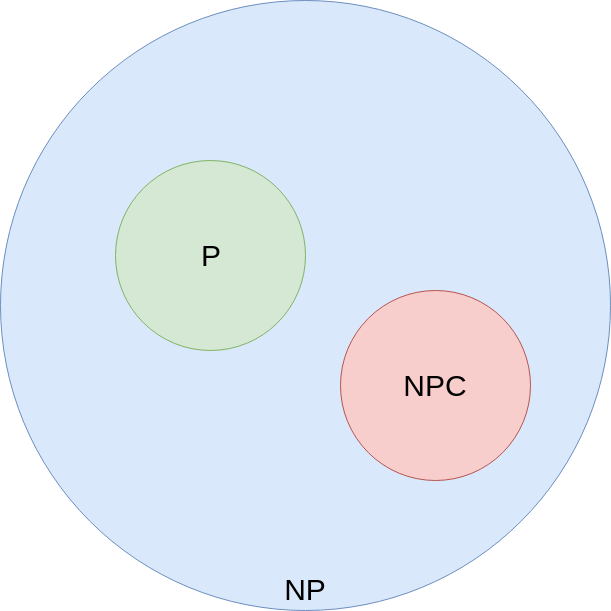
\includegraphics[width=0.5\textwidth]{imgs/np}
	\caption{Venn Diagram of P, NP-Complete, and NP}
	\label{fig:imgs-np}
\end{figure}

\section{Reducibility}%
\label{sec:reducibility}
Example: \\
Subset Sum: Given a set of integers and a target, $t$, is there a subset, $S$ for which $\sum S = t$. \\
Subset Partition: given a set of integers, can they be partitioned into 2 sets with equal sums? \\
\begin{itemize}
	\item If Subset Sum is solved, is it possible to solve subset partition? 
	\item YES! Solve subset sum with $t=\frac{1}{2}\sum S$ where $S$ is all items
	\item We've just used an SS solver to solve SP! This means that SP reduces to SS.
	\item If Instance is "no" in SS, it is also "no" in SP
\end{itemize}

Reducibility: Given problems $L_1$ and $L_2$, we say that $L_1$ is \underline{reducible} to $L_2$ in polynomial time if we can rewrite any instance of $L_1$ as an instance of $L_2$ such that both instances have the same answer. \\

Notation: $L_1 \le L_2$ means that $L_1$ is reducible to  $L_2$. Starting point, $L_1$, is on the left. $SP \le SS$ \\

Example: $HC \le TSP$ \\
Must be able to rewrite HC as TSP such that they have the same answer.
 \begin{figure}[h]
	\centering
	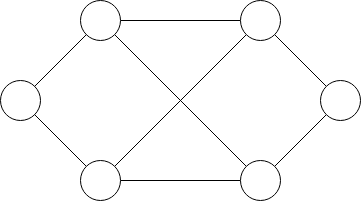
\includegraphics[width=0.6\textwidth]{imgs/hc-tsp}
	\caption{Graph for $HC \le TSP$ Proof}
	\label{fig:imgs-hc-tsp}
\end{figure}

For proof, must be able to show either:
\begin{itemize}
	\item A: $yes \rightarrow yes$ and  $yes \leftarrow yes$
	\item B: $yes \rightarrow yes$ and  $no \rightarrow no$
	\item Either A or B requires two steps
	\item Sometimes one path is much easier
	\item Option B for $HC \le TSP$
	\item If HC is yes instance (HC exists), then the found HC makes TSP a yes instance for weights=1 and bound=num\_nodes
	\item If HC is no instance (no HC exists), then TSP is also no instance because no HCs exist for any cost.
\end{itemize}

\subsection*{Why is Reduction Useful?}
\begin{itemize}
	\item What if SP is intractable, and SS is in P?
	\item This is impossible! Reducibility allows you to solve SP in polynomial-time by transforming into SS and solving.
\end{itemize}

\begin{figure}[h]
	\centering
	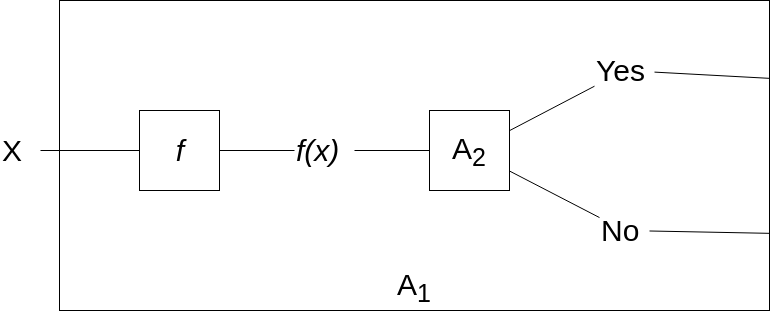
\includegraphics[width=0.8\textwidth]{imgs/reduce}
	\caption{Solving $A_1$ using $A_2$ Solver and Reducibility}
	\label{fig:imgs-reduce}
\end{figure}

\section{NP-completeness}%
\label{sec:np_completeness}

A problem, $L$, is NP-Complete if:
\begin{itemize}
	\item $L \in NP$ 
	\item For every $L' \in NP$, $L' \le L$
\end{itemize}
In words, Every problem in NP should be reducible to L in polynomial time. This essentially means that all NP complete problems are harder than or equal to any other problem in NP. How do we show this? \\

\section{Key Results}%
\label{sec:key_results}

\begin{enumerate}
	\item If $L_1 \le L_2$, and $L_2 \in P$, then $L_1 \in P$
	\item If $L_1 \le L_2$ and $L_1 \notin P$, then $L_2 \notin P$
	\item If $L$ is NPC and $L \in P$, then $NP \in P$
	\item If $L' \in NP$ such that $L' \notin P$, then all $NPC \notin P$
\end{enumerate}

\section{NPC Examples}%
\label{sec:npc_examples_}
\subsection*{Satisfiability (SAT)}
\begin{itemize}
	\item 1971 - Cook found first NPC problem!
	\item Satisfiability Problem (first one!)
	\item Consider boolean expression $\overline{x}_3(x_1+\overline{x}_2+x_3)$ 
	\item Expression is satisfiable if a set of inputs exists which can produce a true output from the expression.
	\item Given a POS form of an expression, is it satisfiable?
	\item Ex: $(x_1+x_2+x_3)(x_1+\overline{x}_2)(x_2+\overline{x}_3)(x_3+\overline{x}_1)(\overline{x}_1+\overline{x}_2+\overline{x}_3)$
	\begin{itemize}
		\item Each clause must be satisfiable
		\item Going by hand from left to right, we can find that this isn't satisfiable.
	\end{itemize}
	\item How can every problem be reduced to this?
	\item All problems in NP have a verification algorithm
	\item Verification algorithm can be expressed as a satisfiability instance, this is the reduction.
	\item This shows that $SAT \in NPC$! First problem ever done.
	\item This result can be leveraged to prove that other problems are NPC
	\item $NP \le SAT$
\end{itemize}

\subsection*{Evolution of Problems}
\begin{itemize}
	\item Year after SAT, first 10 problems shown to be NPC
	\item After 50 years there are TONS of problems in the list of NPC
	\item Problems from every field on here.
	\item When you have a new problem, look for a similar problem that is proved to be NPC and reduce it to your problem.
\end{itemize}

\subsection*{Arbitrary Problem $L_2$}
\begin{itemize}
	\item If $L_1 \in NPC$ and $L_1 \le L_2$ than $L_2 \in NPC$
\end{itemize}

\end{document}
